\documentclass{article}
\usepackage{graphicx}
\usepackage[utf8]{inputenc}
\usepackage[T1]{fontenc}
\usepackage[magyar]{babel}

\usepackage{amsmath}
\usepackage{amsthm}
\usepackage{amssymb}
\usepackage{tikz}
\usepackage{siunitx}
\usepackage{circuitikz}
\usepackage{pgfplots}
\pgfplotsset{compat=1.18}
\usetikzlibrary{arrows.meta, positioning, shapes.geometric}

\theoremstyle{definition}
\newtheorem{definition}{Definíció}

\title{\textbf{Elektromosság}}
\author{Haydu Lőrinc, Rovenszky Robin}
\date{Legutóbb frissítve: 2026. Április 27.}

\begin{document}
\maketitle
\tableofcontents
\vspace{10pt}
\hrule

% ─────────────────────────────────────────────────────────────────────────────
\section{Kezdetek}

\begin{itemize}
    \item Már az ókori görögök felismerték az elektromosság jelenségét
          (pl.\ borostyánkő dörzsölésekor fellépő vonzerő).
    \item Benjamin Franklin írta le először, hogy hogyan keletkeznek a villámok,
          és hogy az elektromosság a fő alkotóelemük.
\end{itemize}

% ─────────────────────────────────────────────────────────────────────────────
\section{Alapok}

\subsection{Elektroszkóp}

Az elektroszkóp az elektromos töltés jelenlétét és relatív nagyságát kimutató
eszköz. Töltött test közelében (vagy érintésre) a belső levelek szétnyílnak,
mert az azonos előjelű töltések taszítják egymást.

\begin{center}
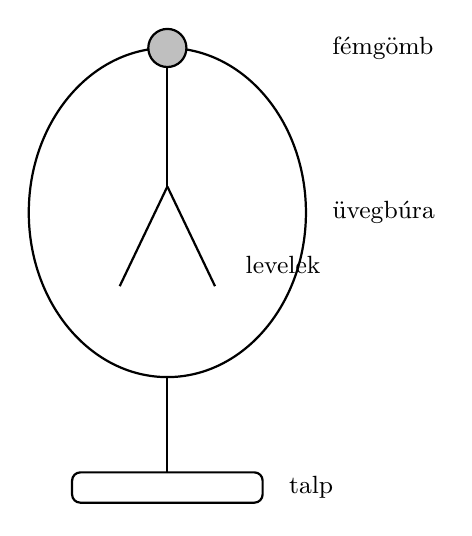
\begin{tikzpicture}[scale=1.1]
    % Glass enclosure (oval bulb)
    \draw[thick] (0,0) ellipse (1.6cm and 1.9cm);
    % Vertical stem
    \draw[thick] (0,-1.9) -- (0,-3.0);
    % Base
    \draw[thick, rounded corners=3pt] (-1.1,-3.0) rectangle (1.1,-3.35);
    % Central metal rod
    \draw[thick] (0, 1.9) -- (0, 0.3);
    % Two leaves (slightly apart)
    \draw[thick] (0, 0.3) -- (-0.55,-0.85);
    \draw[thick] (0, 0.3) -- ( 0.55,-0.85);
    % Top metal knob
    \draw[fill=gray!50, thick] (0, 1.9) circle (0.22cm);
    % Labels
    \node[right=6pt] at (1.6,  1.9) {\small fémgömb};
    \node[right=6pt] at (1.6,  0.0) {\small üvegbúra};
    \node[right=6pt] at (0.6, -0.6) {\small levelek};
    \node[right=6pt] at (1.1, -3.17){\small talp};
\end{tikzpicture}
\end{center}

\begin{definition}[Pozitív töltés]
    A bőrrel dörzsölt üvegrúd töltése. A \emph{pozitív} és \emph{negatív}
    elnevezés csupán konvenció; viszonyítási pontnak a bőrrel dörzsölt üvegrúd
    töltését vesszük.
\end{definition}

% ─────────────────────────────────────────────────────────────────────────────
\subsection{Elektromos áram}

Elektromos áramról akkor beszélünk, ha a töltések \textbf{rendezetten}
mozognak. Ha feltöltünk egy üvegrudat és azzal rohangálunk, az nem rendezett
mozgás — tehát nem áram.

\begin{definition}[Elektromos áram]
    A töltések rendezett mozgása a vezető belsejében.
\end{definition}

\begin{definition}[Egyenáram (DC)]
    Időben \emph{állandó nagyságú} és \emph{állandó irányú} elektromos áram:
    a töltések egy irányban mozognak, az áramerősség értéke nem változik.
\end{definition}

\begin{definition}[Váltóáram (AC)]
    Az áramerősség nagysága és iránya periodikusan változik. A leggyakoribb
    eset a \emph{szinuszos váltóáram}; igazából bármilyen periodikus
    változású áram lehet váltóáram — a szinuszgörbe csak az egyik lehetőség.
\end{definition}

\begin{figure}[h!]
\centering
\begin{tikzpicture}
\begin{axis}[
    width=6.2cm, height=3.5cm,
    xlabel={$t$}, ylabel={$I$},
    xmin=0, xmax=4, ymin=-0.3, ymax=1.7,
    axis lines=left,
    xtick=\empty, ytick={1},
    yticklabels={$I_0$},
    title={\small Egyenáram},
    label style={font=\small},
    tick label style={font=\small},
]
\addplot[thick, blue, domain=0:4] {1};
\end{axis}
\end{tikzpicture}
\hspace{0.8cm}
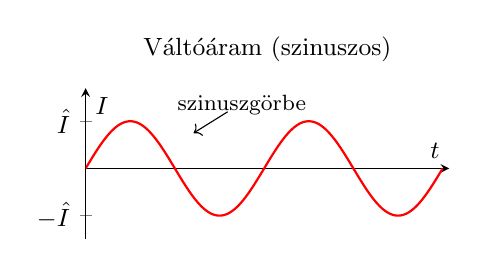
\begin{tikzpicture}
\begin{axis}[
    width=6.2cm, height=3.5cm,
    xlabel={$t$}, ylabel={$I$},
    xmin=0, xmax=12.8, ymin=-1.5, ymax=1.7,
    axis lines=center,
    xtick=\empty, ytick={1,-1},
    yticklabels={$\hat{I}$,$-\hat{I}$},
    title={\small Váltóáram (szinuszos)},
    label style={font=\small},
    tick label style={font=\small},
]
\addplot[thick, red, domain=0:4*pi, samples=200] {sin(deg(x))};
\node[font=\footnotesize] at (axis cs:5.5,1.35) {szinuszgörbe};
\draw[->, thin] (axis cs:5.0,1.2) -- (axis cs:3.8,0.75);
\end{axis}
\end{tikzpicture}
\caption{Egyenáram és szinuszos váltóáram $I$–$t$ diagramja.}
\end{figure}

% ─────────────────────────────────────────────────────────────────────────────
\subsection{Töltéshordozók és vezetési típusok}

A vízben oldott konyhasó $\mathrm{Na^{+}}$ és $\mathrm{Cl^{-}}$ ionokra
esik szét, ezért a sóoldat vezeti az áramot. A desztillált víz — szabad
töltéshordozók hiányában — \emph{nem} vezet.

\begin{definition}[Az áram iránya]
    A pozitív töltésű részecskék mozgásának iránya
    („a pozitív töltések iránya"). Konyhasóoldatban az
    $\mathrm{Na^{+}}$ ionok mozgásának iránya, mivel azok a pozitív
    töltéshordozók — és vice versa a negatív töltésekre.
\end{definition}

Az áram hordozói anyagonként különböznek:

\begin{itemize}
    \item \textbf{Fémes vezetők:} kizárólag \emph{elektronok} mozognak.
          Az elektron negatív töltésű, ezért mozgásiránya
          \emph{ellentétes} az áram konvencionális irányával.
    \item \textbf{Elektrolit oldatok} (pl.\ sóoldat):
          $\mathrm{Na^{+}}$ \emph{és} $\mathrm{Cl^{-}}$ ionok mozognak az
          elektródok felé — a pozitív ionok a katód, a negatív ionok az
          anód felé.
    \item \textbf{Gázok és plazma:} \emph{elektronok és ionok} egyaránt
          részt vesznek a vezetésben.
\end{itemize}

% ─────────────────────────────────────────────────────────────────────────────
\subsection{Áramerősség}

\begin{definition}[Áramerősség ($I$)]
    A vezető keresztmetszetén egységnyi idő alatt átáramló
    töltésmennyiség.
\end{definition}

\[
    I = \frac{Q}{t}
\]

\[
    [I]
    = \frac{\SI{1}{\coulomb}}{\SI{1}{\second}}
    = \underbrace{\SI{1}{\ampere}}_{\text{Amper}}
\]

Az amperóra és a coulomb összefüggése:
\[
    Q = \SI{1}{\ampere\hour} = \SI{3600}{\coulomb}
\]

% ─────────────────────────────────────────────────────────────────────────────
\section{Feszültség és áramkörök}

\subsection{Feszültség}

\begin{definition}[Feszültség ($U$)]
    Az egységnyi pozitív töltés mozgatásához szükséges munka a két pont
    között; megmutatja, mekkora energiát vesz fel (vagy ad le) az
    egységnyi töltés a két pont között.
    \[
        [U] = \underbrace{\SI{1}{\volt}}_{\text{Volt}}
    \]
\end{definition}

Az áram a \emph{magasabb} potenciálú pontból a \emph{kisebb} potenciálú
pont felé folyik. Az áramforrás a kisebb potenciálú végén visszaemeli a
töltések potenciálját — ezáltal a kör záródik, és folyamatos áramlás jön
létre.

\medskip
\noindent\textbf{Megjegyzés:} A feszültség és az áramerősség közötti
összefüggést (Ohm-törvény) a következő alkalommal tárgyaljuk.

% ─────────────────────────────────────────────────────────────────────────────
\subsection{Áramforrások}

\subsubsection{Egyenáramú áramforrások}

\begin{itemize}
    \item \textbf{Ceruzaelem:} \SI{1.5}{\volt}
    \item \textbf{Zsebtelep} (3 db ceruzaelem sorba kötve)\textbf{:}
          \SI{4.5}{\volt}
    \item \textbf{Gombelem:} \SI{3}{\volt}
\end{itemize}

\subsubsection{Váltóáramú áramforrás}

\begin{itemize}
    \item \textbf{Hálózat (konnekt):} szinuszos váltóáramú forrás.
          Effektív feszültség $U_{\mathrm{eff}} = \SI{230}{\volt}$;
          csúcsérték $\hat{U} = 230\sqrt{2} \approx \SI{325}{\volt}$.
\end{itemize}

\begin{center}
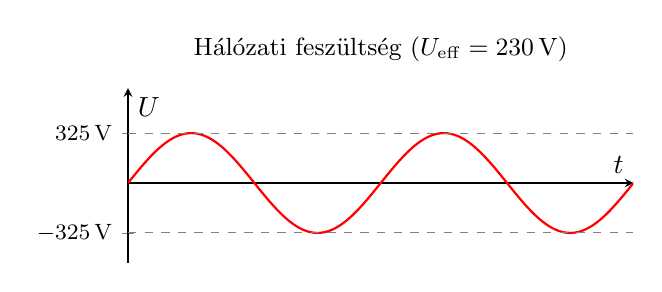
\begin{tikzpicture}
\begin{axis}[
    width=8cm, height=3.8cm,
    xlabel={$t$}, ylabel={$U$},
    xmin=0, xmax=4*pi, ymin=-1.6, ymax=1.9,
    axis lines=center,
    xtick=\empty,
    ytick={1,-1},
    yticklabels={\SI{325}{\volt}, $-$\SI{325}{\volt}},
    tick label style={font=\footnotesize},
    title={\small Hálózati feszültség ($U_{\mathrm{eff}}=\SI{230}{\volt}$)},
    title style={font=\small},
]
\addplot[thick, red, domain=0:4*pi, samples=200] {sin(deg(x))};
\draw[dashed, gray] (axis cs:0,1)  -- (axis cs:4*pi,1);
\draw[dashed, gray] (axis cs:0,-1) -- (axis cs:4*pi,-1);
\end{axis}
\end{tikzpicture}
\end{center}

% ─────────────────────────────────────────────────────────────────────────────
\subsection{Áramkörtípusok}

Az alábbi kapcsolási rajzokon: \quad
\raisebox{-2pt}{\begin{circuitikz}[scale=0.6,transform shape]\draw(0,0) to[battery1](1,0);\end{circuitikz}} = elem, \quad
\raisebox{-4pt}{\begin{circuitikz}[scale=0.6,transform shape]\draw(0,0) to[lamp](1,0);\end{circuitikz}} = lámpa (fogyasztó), \quad
\raisebox{-2pt}{\begin{circuitikz}[scale=0.6,transform shape]\draw(0,0) to[closing switch](1,0);\end{circuitikz}} = kapcsoló.

\subsubsection{Egyszerű zárt áramkör}

Zárt kapcsolónál a kör teljes; áram folyik a fogyasztón át.

\begin{center}
\begin{circuitikz}[scale=1.15, transform shape]
    \draw (0,0) to[battery1, l=elem] (0,2.2)
          to[short]                   (3.5,2.2)
          to[lamp, l=lámpa]           (3.5,0)
          to[short]                   (1.8,0)
          to[closing switch, l=K]     (0,0);
\end{circuitikz}
\end{center}

\subsubsection{Nyitott áramkör}

Nyitott kapcsolónál a kör megszakad; nem folyik áram.

\begin{center}
\begin{circuitikz}[scale=1.15, transform shape]
    \draw (0,0) to[battery1, l=elem] (0,2.2)
          to[short]                   (3.5,2.2)
          to[lamp, l=lámpa]           (3.5,0)
          to[short]                   (1.8,0)
          to[opening switch, l=K]     (0,0);
\end{circuitikz}
\end{center}

\subsubsection{Elágazásos (párhuzamos) áramkör}

Párhuzamos kapcsolásban a feszültség minden ágban azonos.

\begin{center}
\begin{circuitikz}[scale=1.15, transform shape]
    \draw (0,0) to[battery1, l=elem] (0,2.5)
          to[short]      (4,2.5);
    \draw (4,2.5) to[lamp, l=$L_1$] (4,0);
    \draw (2,2.5) to[lamp, l=$L_2$] (2,0);
    \draw (0,0)   to[short]          (4,0);
\end{circuitikz}
\end{center}

\subsubsection{Rövidzárlat}

Rövidzárlatnál az áram a fogyasztót megkerülve, minimális ellenálláson
át záródik. Rendkívül nagy áramerősség keletkezik — \textbf{tűz- és
balesetveszélyes!}

\begin{center}
\begin{circuitikz}[scale=1.15, transform shape]
    \draw (0,0) to[battery1, l=elem] (0,2.2)
          to[short]          (4,2.2)
          to[lamp, l=lámpa]  (4,0)
          to[short]          (0,0);
    % Red short-circuit wire
    \draw[red, very thick] (1.8,2.2) -- node[midway, right, font=\footnotesize, black]
        {rövidzárlat} (1.8,0);
\end{circuitikz}
\end{center}

\end{document}